% Quick start guide
\documentclass{beamer}

\usetheme{Madrid}

% Utilizează biblatex pentru referințe bibliografice
\usepackage[
    maxbibnames=50,
    sorting=nty
]{biblatex}
\usepackage{comment}

\usepackage{fontspec}
% switch to a monospace font supporting more Unicode characters
\setmonofont{FreeMono}
\usepackage{minted}
\newmintinline[lean]{lean4}{bgcolor=white}
\newminted[leancode]{lean4}{fontsize=\footnotesize}
\usemintedstyle{tango}  % a nice, colorful theme

\usepackage{bm}
\usepackage{newunicodechar}
\newunicodechar{ℋ}{$\mathcal{H}$}

\addbibresource{../bibliography.bib}

\usetheme {default}
% Title page details
\title{Mechanizing Many-Sorted Polyadic Hybrid Logic in the Lean 4 Prover}

\author{Andrei-Alexandru Oltean}

\institute{University of Bucharest}

\date{11 September 2025}

\begin{document}

\begin{frame}
    % Print the title page as the first slide
    \titlepage
\end{frame}

\begin{comment}
    \begin{frame}
        \frametitle{Table of Contents}
        \tableofcontents
    \end{frame}
\end{comment}

\begin{frame}
    \frametitle{Mechanizing what?!}
    \begin{itemize}
        \item This 2019 paper \cite{leustean_operational_2019}:
    \end{itemize}
    \centering
        \includegraphics[keepaspectratio=true, height=4cm]{paper.png}
\end{frame}

\begin{frame}[containsverbatim, fragile]
    \frametitle{Mechanizing what?!}

    \begin{center}
        \Large\textbf{%
            \textcolor<1>{gray}{\textcolor<2->{black}{Many-Sorted}} %
            \textcolor<1-2>{gray}{\textcolor<3->{black}{Polyadic}} %
            \textcolor<1-3>{gray}{\textcolor<4->{black}{Hybrid}} %
            \textcolor<1-3>{gray}{\textcolor<4->{black}{Logic}}%
        }
    \end{center}

    \begin{minted}{c}
                s ::= 0;
                i ::= 0;
                while (++i <= n) do
                    s ::= s + i
    \end{minted}
    \begin{align*}
        \uncover<2->{\bm{S} \quad &:= \quad \{ AExp, \; BExp, \; Var, \; Stmt \}} \\
        \uncover<3->{\bm{\Sigma}_{Var,AExp} \quad &:= \quad \{ ++ \} \\
        \bm{\Sigma}_{AExpAExp,AExp} \quad &:= \quad \{ + \} \\
        \bm{\Sigma}_{AExpAExp,BExp} \quad &:= \quad \{ <= \} \\
        \bm{\Sigma}_{VarAExp,Stmt} \quad &:= \quad \{ ::= \} \\
        \bm{\Sigma}_{StmtStmt,Stmt} \quad &:= \quad \{ ; \} \\
        \bm{\Sigma}_{BExpStmt,Stmt} \quad &:= \quad \{ while \; \_ \; do \; \_ \}} \\
        \uncover<4->{\bm{N}_{AExp} \quad := \quad \{ 0 \} \quad & \quad \bm{N}_{Var} \quad := \quad \{ s, \; i, \; n \}}
    \end{align*}

\end{frame}

\begin{frame}[containsverbatim, fragile]
    \frametitle{Mechanizing what?!}

    \begin{center}
        \Large\textbf{
            Many-Sorted Polyadic Hybrid Logic
        }
    \end{center}

    \begin{itemize}
        \item Programming language AST? Or modal logic AST?
    \end{itemize}

    \begin{center}
        \includegraphics[keepaspectratio=true, height=4.5cm]{ast.png}
    \end{center}

    \begin{itemize}
        \item<2-> \textbf{Both.}
    \end{itemize}
\end{frame}

\begin{frame}[containsverbatim, fragile]
    \frametitle{The challenge}

    \begin{enumerate}
        \item<1-> Can we represent such a many-sorted, polyadic grammar in Lean?
        \item<2-> Can we represent its modal semantics?
        \item<3-> Can we prove soundness and completeness of the system?
    \end{enumerate}

    \bigskip

    \pause \pause \pause \pause
    But all this is already done it the paper. What is the point of the Lean implementation? \\
    
    \pause
    \begin{itemize}
        \item<6-> Humans may err; maybe there are errors in the paper;
        \item<7-> The resulting formal artifact could be used as a foundation for verifying software and programming languages in the future.
    \end{itemize}

\end{frame}

\begin{frame}[containsverbatim, fragile]
    \frametitle{What we did}

    \begin{enumerate}
        \item<1-> Implemented the language, its proof system, and its semantics;
        \item<2-> Found and corrected errors in the original axiomatic system;
        \item<3-> Proved soundness of the new system;
        \item<4-> Work is in progress for the completeness proof.
    \end{enumerate}

\end{frame}

\begin{frame}[containsverbatim, fragile]
    \frametitle{The syntax}
    \begin{definition}[Signatures with constant nominals]
        A \textbf{signature with constant nominals} is a triple $(S, \Sigma, N)$, where:
        \begin{itemize}
            \item $S$ is a non-empty, countable set;
            \item $\Sigma$ is an $S^*\times S$-indexed family of countable sets;
            \item $N$ is an $S$-indexed family of non-empty, countable sets.
        \end{itemize}
    \end{definition}

    \pause
    In code:
    \begin{leancode}
        structure Signature (α : Type u) where
            S    : Set α
            «Σ»  : List S → S → Set α
            N    : S → Set α

            sortsCtbl : Encodable S
            opsCtbl (dom range) : Encodable («Σ» dom range)
            nomCtbl (s)         : Encodable (N s)
            sNonEmpty : Inhabited S
    \end{leancode}
\end{frame}

\begin{frame}[containsverbatim, fragile]
    \frametitle{The syntax}
    We further fix sorted sets of propositional variables ($PROP$), non-constant nominals ($NOM$) and state variables ($SVAR$):
    \begin{leancode}
        structure Symbols (α : Type u) where
            signature  : Signature α

            prop : (s : signature.S) → Set α
            nom  : (s : signature.S) → Set α
            svar : (s : signature.S) → Set α

            propCtbl (s) : Encodable (prop s)
            nomCtbl  (s) : Encodable (nom s)
            svarCtbl (s) : Denumerable (svar s)
    \end{leancode}

    \begin{definition}[Formulas]<2->
        The set of formulas is given by the grammar:
        \begin{equation*}
            \varphi_s := p \; | \; j \; | \; y \; | \; \neg \varphi_s \; | \; \varphi_s \lor \varphi_s \; | \; \sigma(\varphi_{s_1}, \dots, \varphi_{s_n}) \; | \; @_k^s \varphi_t \; | \; \forall x \varphi_s,
        \end{equation*}
        \footnotesize
        $p \in PROP_s$, $j \in NOM_s \cup N_s$, $k \in NOM_t \cup N_t$, $y \in SVAR_s$, $x \in SVAR_t$, $\sigma \in \Sigma_{s_1...s_n,s}$
    \end{definition}.
\end{frame}

\begin{frame}[containsverbatim, fragile]
    \frametitle{The syntax}
    In code:
    \begin{leancode}
inductive FormL (symbs : Symbols α) :
    List symbs.signature.S → Type u
| prop : symbs.prop s → FormL symbs [s]
| nom  : symbs.nominal s → FormL symbs [s]
| svar : symbs.svar s → FormL symbs [s]
| appl : symbs.signature.«Σ» (h :: t) s →
            FormL symbs (h :: t) → FormL symbs [s]
| or   : FormL symbs [s] → FormL symbs [s] → FormL symbs [s]
| neg  : FormL symbs [s] → FormL symbs [s]
| at   : symbs.nominal t → FormL symbs [t] → FormL symbs [s]
| bind : symbs.svar t → FormL symbs [s] → FormL symbs [s]
| cons : FormL symbs [s₁] → FormL symbs (s₂ :: t) →
            FormL symbs (s₁ :: s₂ :: t)

abbrev Form (symbs : Symbols α) (s : symbs.signature.S) :=
    FormL symbs [s]
    \end{leancode}
\end{frame}

\begin{frame}[containsverbatim, fragile]
    \frametitle{The semantics}
    In code:
    \begin{leancode}
def Sat (M : Model symbs) (g : Assignment M)
    (w : WProd M.Fr.W sorts) : FormL symbs sorts → Prop
| .prop p        => w ∈ M.Vp p
| .nom n         => w = M.VNom n
| .svar x        => w = g x
| .appl σ arg    => ∃ w', Sat M g w' arg ∧ ⟨w, w'⟩ ∈ M.Fr.R σ
| .neg φ         => ¬ Sat M g w φ
| .or φ ψ        => Sat M g w φ ∨ Sat M g w ψ
| .at k φ        => let u := M.VNom k;  Sat M g u φ
| .bind x φ      => ∀ g', g'.variant g x → Sat M g' w φ
| .cons φ ψs     => Sat M g w.1 φ ∧ Sat M g w.2 ψs
    \end{leancode}
\end{frame}

\begin{frame}[containsverbatim, fragile]
    \frametitle{The proof system}
    Q: Can we take the following schema as an axiom?
    \begin{align*}\tag{Barcan}\label{barcan}
        \vdash^s \forall x \sigma^{\Box}(\varphi_1, \dots, \varphi_n) \to \sigma^{\Box}(\varphi_1,\dots, \forall x \varphi_i, \dots, \varphi_n)
    \end{align*}

    \pause
    No! We found a countermodel:
    \begin{leancode}
theorem BarcanAntecedentTrue  :
    ⟨countermodel, g, w₀⟩ ⊨ barcan_antecedent
theorem BarcanConsequentFalse :
    ⟨countermodel, g, w₀⟩ ⊭ barcan_consequent
    \end{leancode}

    \pause
    We need a restricted version:
    \begin{align*}\tag{Barcan}\label{barcan}
        \vdash^s \forall x \sigma^{\Box}(\varphi_1, \dots, \varphi_n) \to \sigma^{\Box}(\varphi_1,\dots, \forall x \varphi_i, \dots, \varphi_n), \\ \quad \text{ if } x \text{ does not } \text{occur free in } \varphi_j \text{ for } j \neq i
    \end{align*}
\end{frame}

\begin{frame}[containsverbatim, fragile]
    \frametitle{The proof system}
    Q: Can we use the following proof rule?
    \begin{align*}\tag{Name@}\label{Name@}
        \text{If } \vdash^s @_j^s \varphi, \text{then } \vdash^{s'} \varphi, \quad \text{ if } j \text{ does not occur in } \varphi
    \end{align*}

    \pause
    No! Using it on constant nominals leads to unsound derivations. We require:
    \begin{align*}\tag{Name@}\label{Name@}
        \text{If } \vdash^s @_j^s \varphi, \text{then } \vdash^{s'} \varphi, \quad \text{ if } j \not\in N \text{ and } j \text{ does not occur in } \varphi
    \end{align*}
\end{frame}

\begin{frame}[containsverbatim, fragile]
    \frametitle{The proof system}
    Q: Can we use the following proof rule?
    \begin{align*}\tag{Paste}\label{Paste}
        \text{If } \vdash^s @_j \sigma(\dots , k, \dots) \wedge @_k \varphi \to \psi, \text{ then } \vdash^s @_j \sigma(\dots, \varphi, \dots) \to \psi, \\ \quad
            \text{for } k \neq j, \text{ and } k \text{ does not occur in } \varphi \text{ or } \psi
    \end{align*}

    \pause
    Corrected:
    \begin{align*}\tag{Paste}\label{Paste}
        \text{If } \vdash^s @_j \sigma(\dots , k, \dots) \wedge @_k \varphi \to \psi, \text{ then } \vdash^s @_j \sigma(\dots, \varphi, \dots) \to \psi, \\ \quad
            \text{for } k \neq j, k \not\in N, \text{ and } k \text{ does not occur in } \varphi, \psi, \text{ or the } \dots \text{ formulas }
    \end{align*}
\end{frame}

\begin{frame}[containsverbatim, fragile]
    \begin{leancode}
inductive Proof {symbs : Symbols α} (Λ : AxiomSet symbs) :
    (s : symbs.signature.S) → Form symbs s → Type u
  -- Λ:
  | ax    : (φ : Λ s) → Proof Λ s φ
  -- Propositional:
  | prop1 φ ψ   : Proof Λ s (φ ⟶ (ψ ⟶ φ))
  | prop2 φ ψ χ : Proof Λ s ((φ ⟶ (ψ ⟶ χ)) ⟶ (φ ⟶ ψ) ⟶ (φ ⟶ χ))
  | prop3 φ ψ   : Proof Λ s ((∼ψ ⟶ ∼φ) ⟶ (φ ⟶ ψ))
  -- K:
  | k φ ψ χ
      (σ : symbs.signature.«Σ» _ s)
      (C : (φ ⟶ ψ).Context χ):
            Proof Λ s (ℋ⟨σ⟩ᵈ χ ⟶ (ℋ⟨σ⟩ᵈ C[φ] ⟶ ℋ⟨σ⟩ᵈ C[ψ]))
  | mp    : Proof Λ s (φ ⟶ ψ) → Proof Λ s φ → Proof Λ s ψ
  | ug {φ : Form symbs s₁}
       (C : φ.Context ψ):
            Proof Λ s₁ φ → Proof Λ s₂ (ℋ⟨σ⟩ᵈ ψ)
  -- H(@, ∀):
  -- 1. Axioms about @
  | kAt j φ ψ    : Proof Λ s (ℋ@j (φ ⟶ ψ) ⟶ (ℋ@j φ ⟶ ℋ@j ψ))
  | agree j k φ  : Proof Λ s (ℋ@k (ℋ@j φ) ←→ ℋ@j φ)
  | selfDual j φ : Proof Λ s (ℋ@j φ ←→ ∼ ℋ@j (∼φ))
  | intro j φ    : Proof Λ s (ℋNom j ⟶ (φ ←→ ℋ@j φ))
  | back j φ ψ
         (σ : symbs.signature.«Σ» _ s)
         (C : (@FormL.at α symbs t sᵢ j ψ).Context φ):
      Proof Λ s (ℋ⟨σ⟩ φ ⟶ ℋ@j ψ)
  | ref j s₂ : Proof Λ s₂ (ℋ@j (ℋNom j))
  -- 2. Axioms about svars and binders
  | q1 x φ ψ
        (_: φ.occurs_free x = false):
      Proof Λ s (ℋ∀x (φ ⟶ ψ) ⟶ (φ ⟶ ℋ∀x ψ))
  | q2_var (x y: symbs.svarType s') φ:
      φ.free_for y x → Proof Λ s ((ℋ∀x φ) ⟶ φ[y // x])
  | q2_nom (i : symbs.nominal s') (x: symbs.svarType s') φ:
      Proof Λ s ((ℋ∀x φ) ⟶ φ[i // x])
  | name x : Proof Λ s (ℋ∃x (ℋVar x))
  -- 3. Barcan axioms
  | barcan x (φ : Form symbs s)
      (σ : symbs.signature.«Σ» _ s)
      (C : φ.Context ψ)
      (h : C.all_else_not_free x):
            Proof Λ s (ℋ∀x (ℋ⟨σ⟩ᵈ ψ) ⟶ (ℋ⟨σ⟩ᵈ C[ℋ∀x φ]))
  | barcanAt x j φ:
            Proof Λ s (ℋ∀x (ℋ@j φ) ⟶ ℋ@j (ℋ∀x φ))
  -- 4. Axiom Nom, linking svars and nominals together:
  | nom x j k:
            Proof Λ s (ℋ@k (ℋVar x) ⋀ ℋ@j (ℋVar x) ⟶ ℋ@k (ℋNom j))
  -- Hybrid proof rules
  | broadcastS s₂ : Proof Λ s₁ (ℋ@j φ) → Proof Λ s₂ (ℋ@j φ)
  | genAt s₂ j : Proof Λ s₁ φ → Proof Λ s₂ (ℋ@j φ)
  | nameAt s₂ {j : symbs.nominal s₂} {φ : Form symbs s₂} :
            ¬Λ.occurs j → φ.occurs j = false →
            Proof Λ s₁ (ℋ@j φ) → Proof Λ s₂ φ
  | paste (C : (ℋNom k).Context χ):
          k ≠ₛ j → ¬Λ.occurs k → ψ.occurs k = false → C[φ].occurs k = false →
          Proof Λ s (ℋ@j (ℋ⟨σ⟩ χ) ⋀ ℋ@k φ ⟶ ψ) → Proof Λ s ((ℋ@j (ℋ⟨σ⟩ C[φ]) ⟶ ψ))
  | gen x : Proof Λ s φ → Proof Λ s (ℋ∀x φ)
    \end{leancode}
\end{frame}

\begin{frame}[containsverbatim, fragile]
    \frametitle{Soundness and completeness}
    \begin{leancode}
theorem Soundness {Λ : AxiomSet symbs} : ⊢(Λ, s) φ → ⊨Mod(Λ) φ
    \end{leancode}
    Can we do the same for completeness?

    \pause
    Yes, but it's more complex. We took a top-down approach.
\end{frame}

\begin{frame}[containsverbatim, fragile]
    \frametitle{Soundness and completeness}
    State of the completeness formalization:
    \bigskip

    \centering
        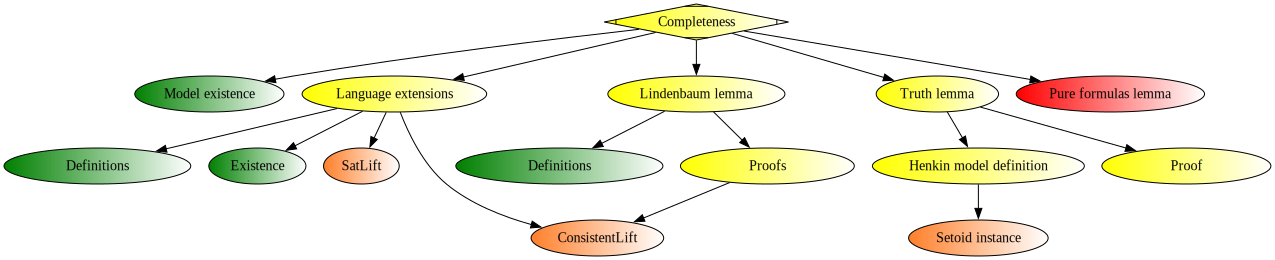
\includegraphics[keepaspectratio=true, width=\textwidth]{completeness.png}
\end{frame}

\begin{frame}[containsverbatim, fragile]
    \frametitle{Future work}

    \begin{enumerate}
        \item<1-> Complete the proof of completeness;
        \item<2-> Formalize applications to PL semantics;
        \item<3-> DSL for seamless specification of PL's.
    \end{enumerate}

\end{frame}

\begin{frame}
    \vspace{1cm}
    \begin{center}
        \Large Thank you!
    \end{center}
\end{frame}

\begin{frame}[allowframebreaks]
    \frametitle{Bibliography}
    \printbibliography
\end{frame}

\end{document}
